% Meta
\documentclass[
  xcolor={svgnames},
  hyperref={
    unicode=true,
    colorlinks=true,
    citecolor=DeepPink,
    linkcolor=DarkRed,
    urlcolor=DarkBlue
  }
]{beamer}

% Fonts
\usepackage[T2A]{fontenc}
\usepackage[utf8]{inputenc}

% Languages
\usepackage[base]{babel}
% Some languages define these commands, so you have to write this to protect yourself from namespace collision errors
\AfterBabelLanguage{bulgarian}{%
  \let\sh\relax\let\ch\relax\let\tg\relax
  \let\arctg\relax\let\arcctg\relax
  \expandafter\let\expandafter\th\csname ltx@th\endcsname
  \let\ctg\relax\let\cth\relax\let\cosec\relax
}
\usepackage[main=bulgarian, english]{babel}
\usepackage{hyphenat}

% Better bibliography
% \usepackage[
%   bibencoding=auto,
%   backend=biber,
%   autolang=other
% ]{biblatex}
\usepackage{natbib}

% Indent first line in paragraph
\usepackage{indentfirst}

% Better math
\usepackage{amsmath}
\usepackage{amsbsy}
\usepackage{amssymb}
\usepackage{mathtools}
\usepackage{comment}
\usepackage{mathptmx}
\usepackage[makeroom]{cancel}

% Better theorems
\usepackage{amsthm}

% Derivative notations
\usepackage{physics}

% Better graphics
\usepackage{subcaption}
\usepackage{graphicx}
%\usepackage{media9}

% Easier element/ion syntax
\usepackage[version=3]{mhchem}

% \usepackage{citation-style-language}
% \cslsetup{style = apa}

\usetheme{Frankfurt}
%\usetheme{Copenhagen}
%\usetheme{Malmoe}
\usecolortheme[named=black]{structure}
\beamertemplatenavigationsymbolsempty



\title{Моделиране на нервни импулси}
\subtitle{Проект по "Семинар по математическо моделиране"}
\author{изготвил: Калоян Стоилов}
\institute{Софийски университет "Св. Климент Охридски" \\ Факултет по математика и информатика}
\institute{\textbf{\textit{СОФИЙСКИ УНИВЕРСИТЕТ \\ "СВ. КЛИМЕНТ ОХРИДСКИ"}}
  \begin{center}
    
\includegraphics[width=1.2cm,height=1.5cm]{img/logo_su}
  \end{center}
  ФАКУЛТЕТ ПО МАТЕМАТИКА И ИНФОРМАТИКА
}

% Roman numerals for sections
\renewcommand{\thesection}{\Roman{section}}

% Numbering of equations
\newcommand\numberthis{\addtocounter{equation}{1}\tag{\theequation}}
\renewcommand{\theequation}{\Roman{section}.\arabic{equation}}

% Space between lines in array for fractions
\renewcommand{\arraystretch}{1.5}

% Some stupid thing due to adding more than one language in babel and having to specify main
\ifx\bulgarianhyphenmins\undefined
\def\bulgarianhyphenmins{2 2}
\fi

% Bibliography resourse
% \setbeamertemplate{bibliography entry title}{}
% \setbeamertemplate{bibliography entry location}{}
% \setbeamertemplate{bibliography entry note}{}

% Bibliography resourse
% \makeatletter
%   \@ifpackageloaded{biblatex}
%     {\addbibresource{neurons.bib}}
%     {\bibliography{neurons}}
% \makeatother
%\addbibresource[bibencoding=utf8]{neurons.bib}

%\setbeamertemplate{headline}[default]
% \setbeamertemplate{headline}
% {%
% \begin{beamercolorbox}{}
% \insertpagenumber
% %\vskip2pt\insertnavigation{\paperwidth}\vskip2pt
% \end{beamercolorbox}%
% }
\setbeamertemplate{headline}{}
\setbeamertemplate{footline}[frame number]

\begin{document}
\nocite{*}
{

  \begin{frame}[noframenumbering, plain]
    \titlepage
  \end{frame}

}

\begin{frame}[t]{Хистология на нервната тъкан}
  В нервната тъкан има два основни вида клетки - неврони и глиоцити.
  Електрични импулси се предават по невроните, а (невро-)глията,
  както понякога се нарича съвкупността от глиоцити, подпомага тяхната работа.

  От нервна тъкан е изградена нервната система, която се дели на централна (гръбначен мозък и главен мозък) и периферна (соматична и автономна).
\end{frame}

\begin{frame}[t]{Невроглия}
  Глиоцитите могат да участват в митоза, т.е. да се делят. "Най-важните" видове невроглия са:
  \begin{enumerate}
    \item Астроцити - връзка между невроните и кръвта
    \item Олигодендроцити - покриват аксоните на невроните в централната нервна система, образувайки миелинова обвивка, която действа като диелектрик
    \item Шванови клетки - подобни на олигодендроцитите, но в периферната нервна система
    \item Радиална глия - отговарят за неврогенезата и синаптичната пластичност
    \item Микроглия - имунна защита
  \end{enumerate}
\end{frame}

\begin{frame}[t]{Неврони}
  Невроните не участват в митоза. Функционално могат да се разделят на три типа
  \begin{enumerate}
    \item Аферентни (рецептори) - носят информация за околния свят
    \item Интерневрони (конектори) - свързват различни региони на мозъка, позволяват рефлексите и обучението
    \item Еферентни (моторни) - активират мускули и жлези
  \end{enumerate}
\end{frame}

\begin{frame}[t]{Хистология на нервната тъкан}
  \begin{figure}[htbp!]
    \centering
    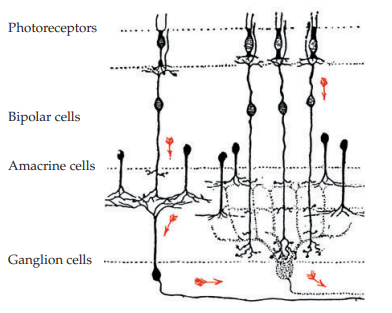
\includegraphics[width=\textwidth,height=0.7\textheight,keepaspectratio]{img/neuron/complex.PNG}
    \caption{Структура и връзки между клетките на ретината при бозайници. \cite[Фиг 1.2]{Neuron}}
  \end{figure}
\end{frame}

\begin{frame}[t]{Хистология на нервната тъкан}
  \begin{figure}[htbp!]
    \centering
    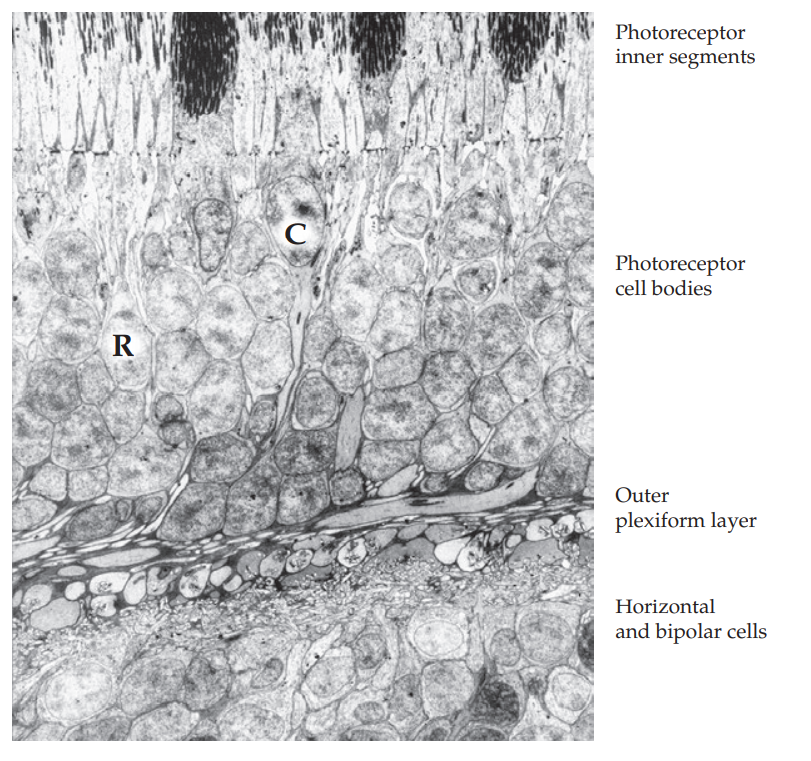
\includegraphics[width=\textwidth,height=0.7\textheight,keepaspectratio]{img/neuron/macaque.PNG}
    \caption{Електромикроскопска снимка на ретина на макак. \cite[Фиг 1.3]{Neuron}}
  \end{figure}
\end{frame}

\begin{frame}[t]{Хистология на нервната тъкан}
  \begin{figure}[htbp!]
    \centering
    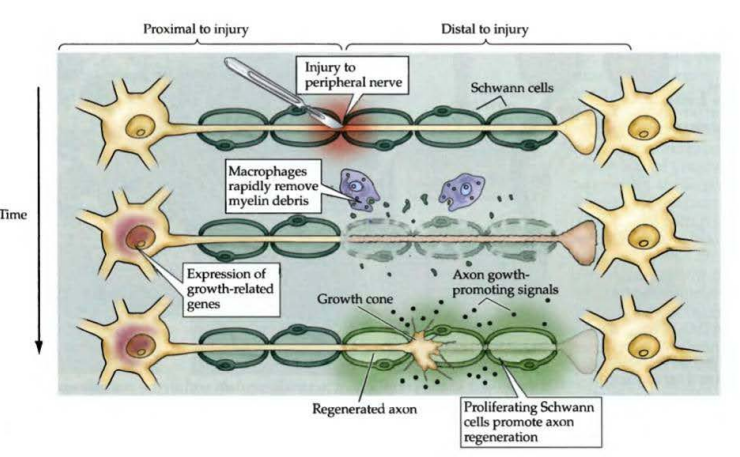
\includegraphics[width=\textwidth,height=0.7\textheight,keepaspectratio]{img/axon/regeneration.PNG}
    \caption{Регенерация на аксон в ПНС \cite[Фиг 25.5]{Neuroscience}}
  \end{figure}
\end{frame}

\begin{frame}[t]{Морфология на невроните}
  \begin{enumerate}
    \item   Дендрити - разклонявания на клетната, в краищата на които бива въздействана от други неврони
    \item   Сома - "основната" част на клетката, включваща ядрото и повечето органели
    \item   Аксон - къс (в ЦНС) или дълъг (в ПНС) израстък, служещ за предаване на импулси към други клетки
    \item   Телодендрия - разколявания на аксона в края му
    \item   Синапс - окончание на разклоненията. 
    \begin{enumerate}
      \item   Електрични синапси - сдвояване на клетки
      \item   Химични синапси - контакът се извършва непряко чрез невротрансмитери
    \end{enumerate}
    \item   Прищъпване на Ранвие - участък между два миелинови участъка
  \end{enumerate}
\end{frame}
\section{Физиология}
\begin{frame}[t]{Физиология на невроните}
  Поддържане на различна концентрация на йони в цитозола спрямо околната тъкан.
  \ce{K+} и някои белтъци с общ отрицателен заряд са с по-голяма концентрация в клетката,
  докато \ce{Na+} и \ce{Cl-} извън нея. Това води до създаването на тъй наречения (транс-)мембранен потенциал.
  Клетъчната мембрана се състои основно от липиди, чиято хидрофобна част се държи като диелектрик.
  Липидната част на мембраната всъщност се оказва кондензатор.
  Предвижването на йони през мембраната става чрез помпи (активно) и канали (пасивно).
  Основни са тъй наречените натриево-калиевите помпи, това са молекули \ce{Na-K-ATPase}. Те предвижват 3 \ce{Na+} йона навън и 2 \ce{K+} навътре.
  Други важни помпи са натриево-калциевите, като предвижват 1 \ce{Ca2+} йон навън и 3 \ce{K+} навътре.
\end{frame}

\begin{frame}[t]{Причината за трансмембранния потенциал}
  \begin{figure}[htbp!]
    \centering
    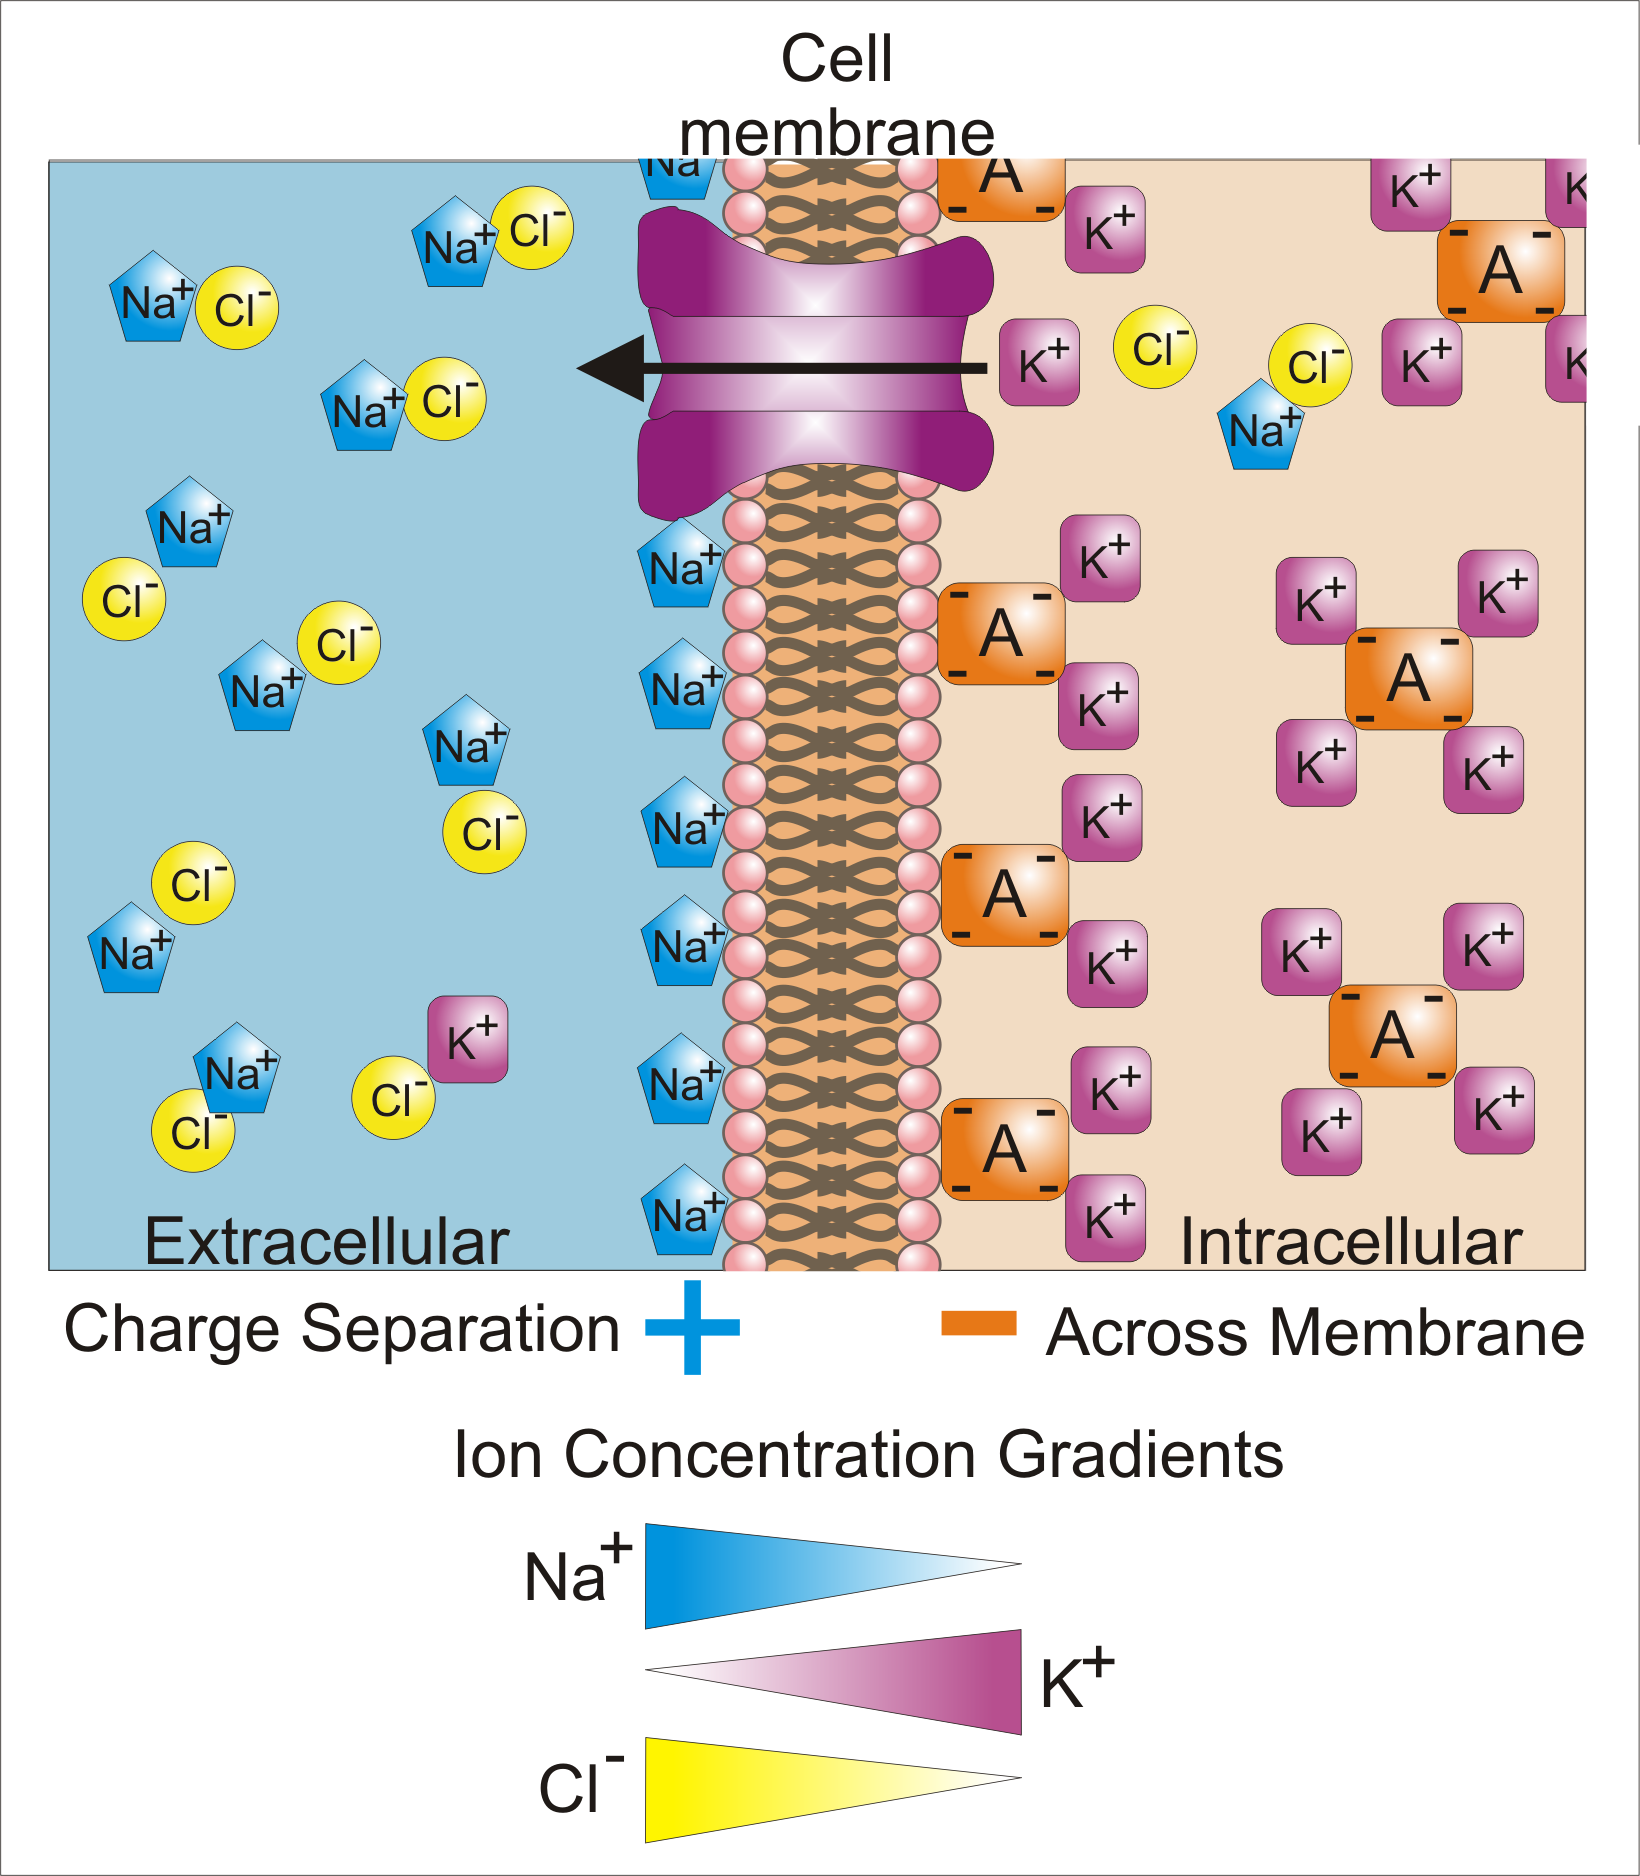
\includegraphics[width=\textwidth,height=0.7\textheight,keepaspectratio]{img/activation/membrane-potential.png}
    \caption{Йони в цитозола и междуклетъчното пространство от Wikipedia}
  \end{figure}
\end{frame}

\begin{frame}[t]{Физиология на невроните}
  \begin{figure}[htbp!]
    \centering
    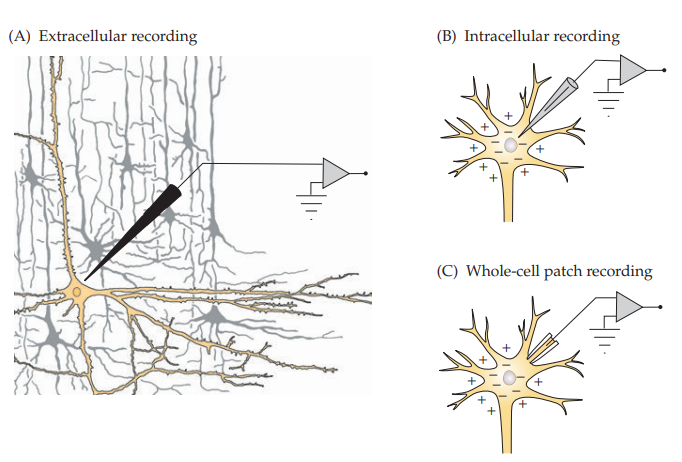
\includegraphics[width=\textwidth,height=0.7\textheight,keepaspectratio]{img/activation/electrical-recording.PNG}
    \caption{Измерване на потенциала. \cite[Фиг 1.7]{Neuron}}
  \end{figure}
\end{frame}

\begin{frame}[t]{Физиология на невроните}
  \begin{figure}[htbp!]
    \centering
    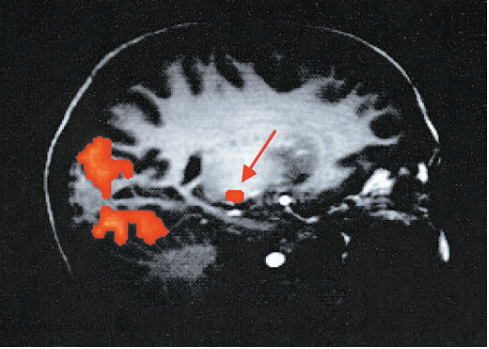
\includegraphics[width=\textwidth,height=0.7\textheight,keepaspectratio]{img/activation/mri-recording.PNG}
    \caption{Измерване на активността на невроните в главния мозък чрез ЯМР. \cite[Фиг 1.9]{Neuron}}
  \end{figure}
\end{frame}

\begin{frame}[t]{Междуневронна комуникация}
  Предаването на сигнали между неврони става през синапсите.
  При електричните синапси става директно, едната клетка "продължава" в другата.
  При химичните синапси се образуват везикули (балончета с вещества) в синаптичния цитозол,
  които се придвижват до мембраната и освобождават вътрешността си в междуклетачното пространство.
  В резултат следващия неврон може или да бъде възбуден, или инхибиран.
\end{frame}

\begin{frame}[t]{Междуневронна комуникация}
  \begin{figure}[htbp!]
    \centering
    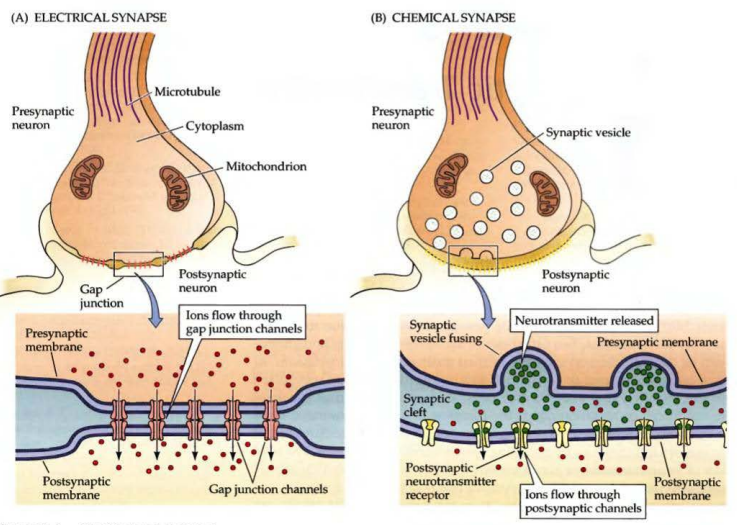
\includegraphics[width=\textwidth,height=0.7\textheight,keepaspectratio]{img/activation/synapse-types.PNG}
    \caption{Двата вида синапси. \cite[Фиг 5.1]{Neuroscience}}
  \end{figure}
\end{frame}

\begin{frame}[t]{Междуневронна комуникация}
  \begin{figure}[htbp!]
    \centering
    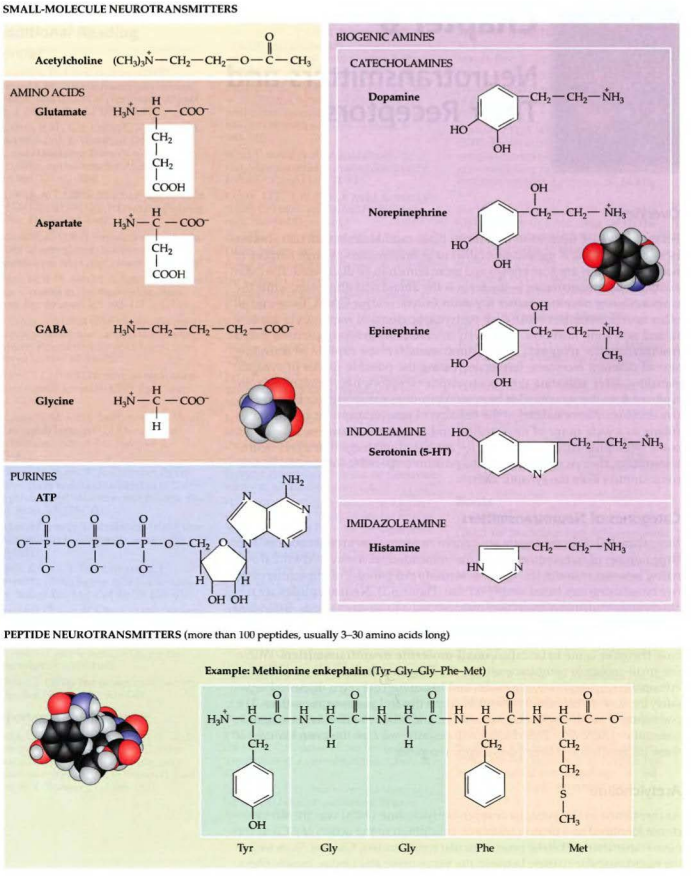
\includegraphics[width=\textwidth,height=0.7\textheight,keepaspectratio]{img/activation/neurotransmitters.PNG}
    \caption{Молекулите на някои невротрансмитери. \cite[Фиг 6.1]{Neuroscience}}
  \end{figure}
\end{frame}

\begin{frame}[t]{Междуневронна комуникация}
  \begin{figure}[htbp!]
    \centering
    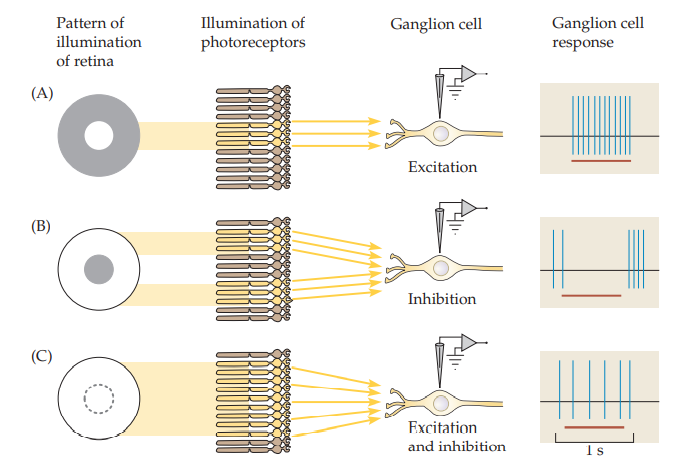
\includegraphics[width=\textwidth,height=0.7\textheight,keepaspectratio]{img/activation/gangleon-integration.PNG}
    \caption{Интегриране от ганглийна клетка. \cite[Фиг 1.16]{Neuron}}
  \end{figure}
\end{frame}

\begin{frame}[t]{Нервен импулс}
  \begin{figure}[htbp!]
    \centering
    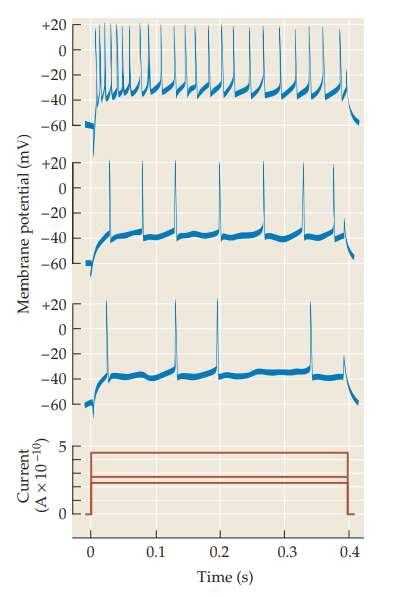
\includegraphics[width=\textwidth,height=0.7\textheight,keepaspectratio]{img/activation/ac-current.PNG}
    \caption{Резултат от подаване на прав ток чрез електрод в цитозола на ретинална ганглийна клетка. \cite[Фиг 1.12]{Neuron}}
  \end{figure}
\end{frame}

\begin{frame}[t]{Причина за нервния импулс}
  Нервният импулс е резултат от каскадно действие на мембранните канали и помпи.
  Първо клетката се активизира.
  Ако е рецептор, то тя се възбужда от околната среда.
  В противен случай възбудата става в следствие на получени невротрансмитери от дендритите.
  След леко повишаване на трансмембранния потенциал се отключват \ce{Na+} канали, чиято ориентация зависи от потенциала.
  Те са открити благодарение на изследванията на Alan Hodgkin и Andrew Huxley върху \textit{Doryteuthis pealeii} (вид сепия).
  %В клетката излизат \ce{Ca2+} и влизат \ce{Na+}, което води до промяна на потенциала и активиране на \ce{Na+} канали, зависими от него.
  %\ce{Na-K-ATPase}.
  %Това води до още промяна на потенциала в околност на натриево-калиевата помпа, което активира други около нея.
\end{frame}

\begin{frame}[t]{Причина за нервния импулс}
  \begin{figure}[htbp!]
    \centering
    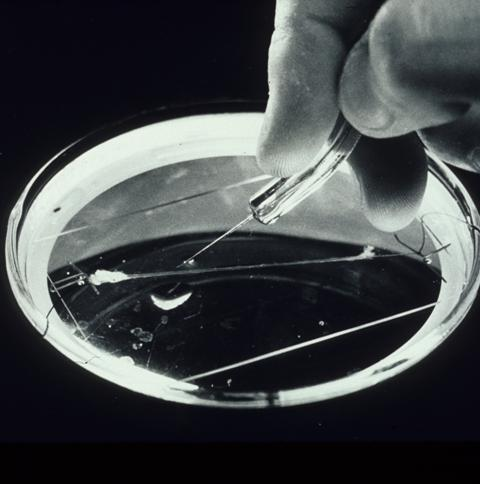
\includegraphics[width=\textwidth,height=0.7\textheight,keepaspectratio]{img/axon/squid.jpg}
    \caption{Гигантския сепиен аксон от Wikipedia}
  \end{figure}
\end{frame}

\begin{frame}[t]{Причина за нервния импулс}
  Така потенциалът се увеличава още повече и се активизират други канали в околността.
  Включват се и канали, позволяващи преминаването на \ce{K+} навън.
  След деполяризация каналите се затварят.
  \ce{Na-K-ATPase} се грижи концентрациите на йоните да се възвърнат първоначалните си стойности.
  Така потенциалът се понижава до достигане (и леко прехвърляне) на стойността му в покой.
  Накрая бавно се достига равновесното състояние.
\end{frame}

\begin{frame}[t]{Причина за нервния импулс}
  \begin{figure}[htbp!]
    \centering
    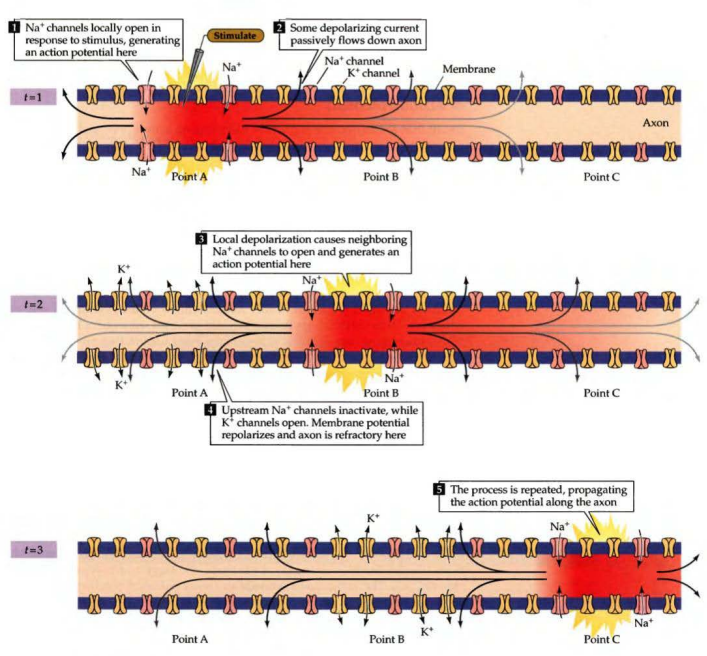
\includegraphics[width=\textwidth,height=0.7\textheight,keepaspectratio]{img/axon/bare.PNG}
    \caption{Разпространение на нервния импулс \cite[Фиг 3.12]{Neuroscience}}
  \end{figure}
\end{frame}

\begin{frame}[t]{Причина за нервния импулс}
  \begin{figure}[htbp!]
    \centering
    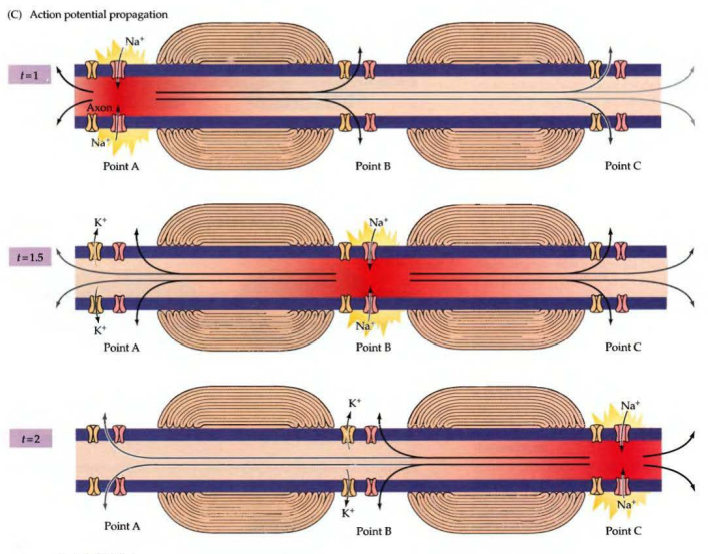
\includegraphics[width=\textwidth,height=0.7\textheight,keepaspectratio]{img/axon/myelin.PNG}
    \caption{Влиянието на миелиновата обвивка върху нервния импулс \cite[Фиг 3.13]{Neuroscience}}
  \end{figure}
\end{frame}

\begin{frame}[t]{Причина за нервния импулс}
  \begin{figure}[htbp!]
    \centering
    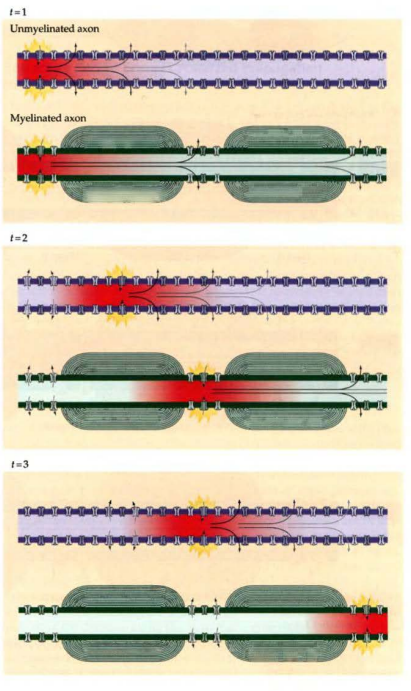
\includegraphics[width=\textwidth,height=0.7\textheight,keepaspectratio]{img/axon/comparison.PNG}
    \caption{Сравнение на скоростите на протичане на импулса \cite[Фиг 3.14]{Neuroscience}}
  \end{figure}
\end{frame}

\begin{frame}[t]{Миелинова обвивка}
  Пасивният поток на електричния ток се извършва без необходима енергия на клетката.
  Напрежението на разстояние от $x$ от място, където се подава ток, се изразява чрез:
  \begin{equation*}
    V_x=V_0 e^{-\frac{x}{\lambda}}, \quad \lambda=\sqrt{\frac{r_m}{r_o+r_i}}
  \end{equation*}
  Където $r_m$ е съпротивлението на мембраната, $r_o$ - на междуклетачното пространство, а $r_i$ - на аксоплазмата (цитоплазмата в аксона).
  Олигодендроцитите/Швановите клетки са закрепени за аксона и премахват ефекта на междуклетъчното пространство.
  Миелинът е повишаващ съпротивлението участник.
\end{frame}

\begin{frame}[t]{Уравнение на Nernst}
    Уравнения на Nernst се използват в $RedOx$ процеси, като се изразява промяна в енергията на Гибс $G$ като:
    \begin{align*}
        &-zFE_{cell} = \Delta G = -RT \ln K \\
        &\implies E_{cell} = \frac{RT}{zF} \ln K
    \end{align*}
    Тук $R$ е универсалната газова константа, $T$ - температурата, $K$ - равновесната константа на процеса,
    $F$ - константа на Фарадей (заряда на 1 мол електрони), $zF$ е размера на заряда, обменен по време на реакцията.
\end{frame}

\begin{frame}[t]{Уравнение на Goldman-Hodgkin-Katz}
    Желаем да изразим трансмембранно напрежение $V_m$, с оглед на симетричност е достатъчно да разглеждаме едномерна задача по права, нормална на мембраната.
    Допускаме, че йон $\mathrm{A}$ с валентност $n_A$ през мембрана с дебелина $L$, като нека оста $z$ е нормална на мембраната и съответно $\left[\mathrm{A}\right]=\left[\mathrm{A}\right](z)$. 
    На това съответства поток $j_A$. Част от него се описва чрез дифузията $-D_{\mathrm{A}}\dv{\left[{\mathrm{A}}\right]}{z}$ по закона на Фик.
    Той ни казва, че от Брауновото движение $\mathrm{A}$ се движи натам, където има по-малка концентрация.
    Останалата част идва от $D_{\mathrm{A}}\frac{n_{\mathrm{A}}F}{RT}\frac{V_m}{L}\left[\mathrm{A}\right]$. 
    Това следва от закон на Айнщайн за изразяване на коефициента на дифузия.
\end{frame}   

\begin{frame}[t]{Уравнение на Goldman-Hodgkin-Katz}
    Виждаме, че се получава ОДУ от 1-ви ред за $\left[\mathrm{A}\right]$. След решаване и изразяване на потока чрез нея, имаме:
    \begin{align*}
        &\left[\mathrm{A}\right](0) = \left[\mathrm{A}\right]_{in} &\left[\mathrm{A}\right](L) = \left[\mathrm{A}\right]_{out} \\
        &j_{\mathrm {A}}=\mu n_{\mathrm {A}}P_{\mathrm{A}}{\frac{\left[\mathrm{A}\right]_{\mathrm {out}}-\left[\mathrm {A}\right]_{\mathrm{in}}e^{n_{\mathrm {A}}\mu}}{1-e^{n_{\mathrm {A}}\mu}}} \\
        &\mu=\frac{FV_m}{RT} &P_{\mathrm{A}}=\frac{D_{\mathrm {A}}}{L}\\
    \end{align*}
\end{frame}

\begin{frame}[t]{Уравнение на Goldman-Hodgkin-Katz}
    Нека сега $J_{\mathrm{A}}=q_{\mathrm{A}}j_{\mathrm{A}}$ - това е плътността на електричен заряд.
    Но при $V_m$ пълната плътност на заряда трябва да е 0. Тогава ако означим 
    \begin{align*}
        &v=\sum_{{{\mathrm{cations\ C}}}}P_{{{\mathrm{C}}}}\left[{\mathrm{C}}^{{+}}\right]_{{{\mathrm{in}}}}+\sum_{{{\mathrm{anions\ A}}}}P_{{{\mathrm{A}}}}\left[{\mathrm{A}}^{{-}}\right]_{{{\mathrm{out}}}} \\
        &w=\sum_{{{\mathrm{cations\ C}}}}P_{{{\mathrm{C}}}}\left[{\mathrm{C}}^{{+}}\right]_{{{\mathrm{out}}}}+\sum_{{{\mathrm{anions\ A}}}}P_{{{\mathrm{A}}}}\left[{\mathrm{A}}^{{-}}\right]_{{{\mathrm{in}}}} 
    \end{align*}
    То е в сила $w - v e^\mu = 0 \implies \mu = \ln \frac{w}{v} \implies V_m = \frac{RT}{F} \ln \frac{w}{v}$. 
\end{frame}
\begin{frame}[t]{Модел на Hodgkin-Huxley}
  Вече казахме, че липидната част на мембраната действа като кондензатор с капацитет $C$. 
  Помпите може да разглеждаме като проводници със съответна проводимост $g_{Na}$ и $g_{K}$.
  Проводимостта е обратнопропорционална на съпротивлението, 
  т.е. все едно това са резистори със съпротивления $\frac{1}{g_{Na}}$, $\frac{1}{g_{K}}$.
  Може да направим усложнение - $g_{l}$ проводимост на изтичащи йони от каналите. 
\end{frame}

\begin{frame}[t]{Модел на Hodgkin-Huxley}
  \begin{figure}[htbp!]
      \centering
      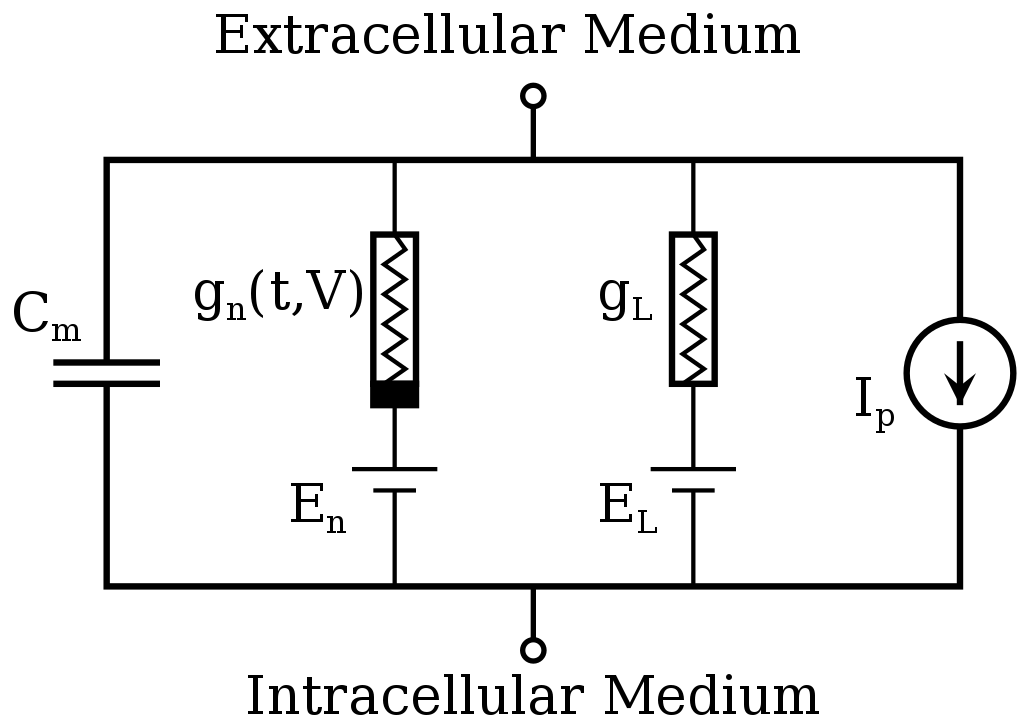
\includegraphics[width=\textwidth,height=0.7\textheight,keepaspectratio]{img/hodgkin-huxley/circuit.png}
      \caption{Еквивалентна електрическа верига от Wikipedia}
  \end{figure}
\end{frame}

\begin{frame}[t]{Модел на Hodgkin-Huxley}
  Да припомним, че $I = \dv{q}{t}$. 
  Сега може да изразим по дефиниция $C$ чрез моментните заряд $q$ и мембранния потенциал $V_m$, т.е. $C = \frac{q}{V}$.
  Откъдето $q = C V$ и $I_C = \dv{C V_m}{t} = \dv{C}{t}V_m + C\dv{V_m}{t}$. 
  Допускаме, че капацитета на мембраната не се променя с времето и достигаме до $I_C = C\dv{V}{t}$.
  Общия ток е сумата от 4-те тока, т.е.:
  \begin{equation*}
    I=C_{m}\dv{V_m}{t}+g_{K}(V_{m}-V_{K})+g_{Na}(V_{m}-V_{Na})+g_{l}(V_{m}-V_{l})
  \end{equation*}
\end{frame}

\begin{frame}[t]{Модел на Hodgkin-Huxley}
  От експериментите си върху аксона на сепия, Hodgkin и Huxley достигнали до следните изрази за пропускливостите:
  \begin{align*}
    &g_{K}=\tilde{g}_{K}n^4,\quad &g_{Na}=\tilde{g}_{Na}m^3h \\
    &\dv{p}{t}=\alpha_p(V_m)(1-n)-\beta_p(V_m)p,\quad &p={n,m,h}
  \end{align*}
  Тук $\tilde{g}_{K}$ и $\tilde{g}_{Na}$ са съответните максимални стойности на пропускливостта.
  Фунцкиите $\alpha_p$ и $\beta_p$ са експериментално установени като: 
  \begin{align*}
    &\alpha_{n}(V_{m})={\frac{0.01(10-V)}{\exp\left({\frac{10-V}{10}}\right)-1}} &\beta_{n}(V_{m})=0.125\exp\left(-\frac{V}{80}\right)\\
    &\alpha_{m}(V_{m})={\frac{0.1(25-V)}{\exp\left({\frac{25-V}{10}}\right)-1}} &\beta_{m}(V_{m})=4\exp\left(-\frac{V}{18}\right)\\
    &\alpha_{h}(V_{m})=0.07\exp\left(-{\frac{V}{20}}\right) &\beta_{h}(V_{m})={\frac{1}{\exp\left({\frac{30-V}{10}}\right)+1}}  
  \end{align*}
  Тук $V = V_{equilibrium} - V_m$.
\end{frame}

\begin{frame}[t]{Модел на Hodgkin-Huxley}
  Нека $a$ е радиусът на аксона, $R$ съпротивлението на цитоплазмата, а $x$ е ос по дължината на аксона.
  Може да се покаже, че $I={\frac{a}{2R}}\pdv[2]{V}{x}$, чрез тъй нареченото кабелно уравнение.
  Така за $V$ получаваме ЧДУ от тип реакция-дифузия.
  Моделът може да се усложни и за повече на вид йони, но трябва емпирично да се намерят изрази за съответстващите им пропускливости.

  Смисълът на $n$ е, че определя до колко са отворени \ce{K+} каналите.
  Аналогично $m$ и $h$ действат като активатор/деактиватор на \ce{Na+} каналите.
\end{frame}

\begin{frame}[t]{Модел на Hodgkin-Huxley}
  \begin{figure}[htbp!]
      \centering
      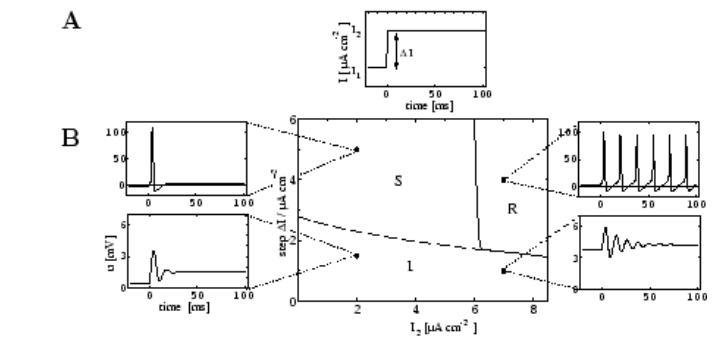
\includegraphics[width=\textwidth,height=0.7\textheight,keepaspectratio]{img/hodgkin-huxley/response.PNG}
      \caption{Подаване на стъпаловиден ток на модела на Hodgkin-Huxley, т.че $I_2$=$I_1$+$\Delta I$ \cite[Фиг 2.6]{Spiking}}
  \end{figure}
\end{frame}

% \begin{frame}[t]{Модел на Hodgkin-Huxley}
%   \begin{figure}[htbp!]
%       \centering
%       %\includemovie{1cm}{1cm}{hodgkin-huxley-graph.gif}
%       %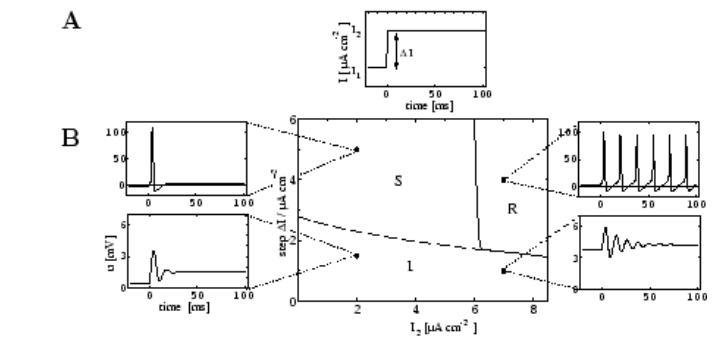
\includegraphics[width=\textwidth,height=0.7\textheight,keepaspectratio]{hodgkin-huxley-response.PNG}
%       %\animategraphics{12}{hodgkin-huxley-graph/54223cdddc0944ffde281cbf29a5bf157wMigNej1EKKnEa6-}{0}{17}
%       %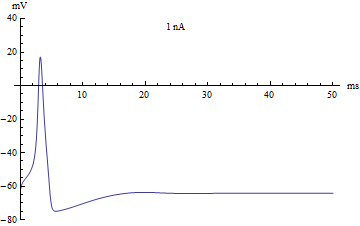
\includegraphics[width=\textwidth,height=0.7\textheight,keepaspectratio]{img/hodgkin-huxley/graph/54223cdddc0944ffde281cbf29a5bf157wMigNej1EKKnEa6-6.png}
%       %\includegraphics[width=\textwidth,height=0.7\textheight,keepaspectratio]{img/hodgkin-huxley/graph-6.png}
%       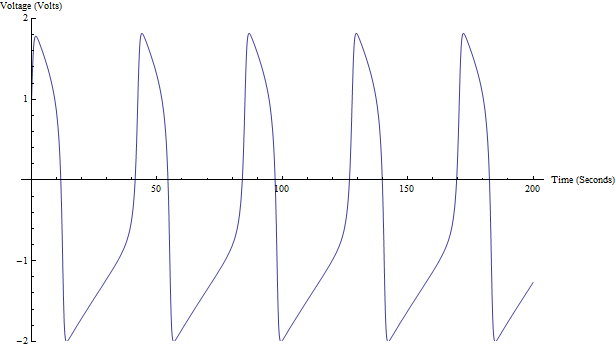
\includegraphics[width=\textwidth,height=0.7\textheight,keepaspectratio]{img/hodgkin-huxley/graph.gif}
%       \caption{Симулация на модела на Hodgkin-Huxley от Wikipedia}
%   \end{figure}
% \end{frame}
\begin{frame}[t]{Модел на FitzHugh-Nagumo}
  Моделът на FitzHugh-Nagumo се стреми да улесни пресмятането на трансмембранния потенциал за сметка на точността.
  \begin{align*}
    &\dv{v}{t} = v - \frac{v^{3}}{3} - w + I_{\rm{ext}} \\
    &\dv{w}{t} = \frac{1}{c}\left(v + a - bw\right)
  \end{align*}
  Тук $w$ е възвръщаша променлива с цел бавен feedback. 
  $I_{\rm{ext}}$ е стимулиращ неврона ток.
  Nagumo съпоставил следната електрическа верига:
\end{frame}

\begin{frame}[t]{Модел на FitzHugh-Nagumo}
  \begin{figure}[htbp!]
    \centering
    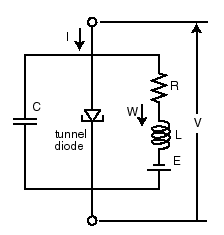
\includegraphics[width=\textwidth,height=0.7\textheight,keepaspectratio]{img/fitzhugh-nagumo/circuit.png}
    \caption{Еквивалентна верига на модела на FitzHugh-Nagumo от Scholarpedia}
  \end{figure}  
\end{frame}

\begin{frame}[t]{Модел на FitzHugh-Nagumo}
  \begin{figure}[htbp!]
    \centering
    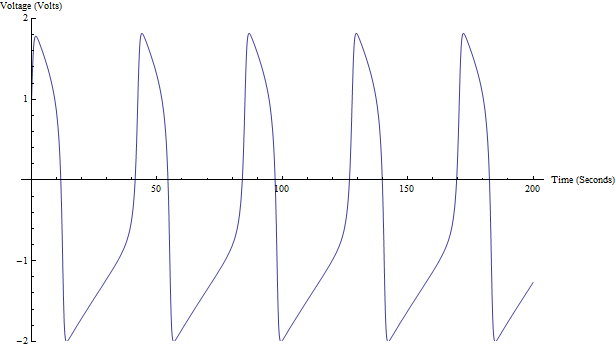
\includegraphics[width=\textwidth,height=0.7\textheight,keepaspectratio]{img/fitzhugh-nagumo/graph.png}
    \caption{Симулация на модела на FitzHugh-Nagumo от Wikipedia}
  \end{figure}  
\end{frame}
\input{hindmarsh–rose}

{
  \begin{frame}[t]{Източници}
    \scriptsize{\bibliographystyle{plainnat}}
    \bibliography{neurons}
    %\bibliographystyle{amsalpha}
    %\printbibliography
    %\bibliography{neurons.bib}
    %\printbibliography
  \end{frame}

  \begin{frame}
    \begin{center}
      \textbf{Благодаря за вниманието}
    \end{center}
  \end{frame}
}

\end{document}
